\documentclass{article}
\usepackage[utf8]{inputenc}
\usepackage[T2A]{fontenc}
\usepackage[russian,english]{babel}
\usepackage{ragged2e}
\usepackage{graphicx} % Required for inserting images
\usepackage{tabularx}
\usepackage{amsmath}

\newtheorem{theorem}{Теорема}

\newtheorem{definition}{Определение}[section]

\graphicspath{{.}}

\title{Задание по курсу "ВвЧМ 24/25": Приближение функций}
\author{Павел Васильев, 213 группа}
\date{Декабрь 2024}

\begin{document}

\maketitle

\section{Постановка задачи}
Интерполяция - это способ нахождения промежуточных значений величины по имеющемуся дискретному набору известных значений.

Перечисленные ниже методы предназначены для создания ряда с более высокой частотой наблюдений на основе ряда с низкой частотой. Например, вычислить ряд с квартальной динамикой на основе ряда годовых данных.

Многие задачи машинного обучения можно сформулировать через интерполяцию "неизвестной" функции [1, 2]

Различные методы численного приближения и их теоретические обоснования можно найти в [3]

\subsection{Условия задачи}
Построить полином Лагранжа для следующих функций \(f_i(x)\) на отрезке \(x \in [-2,0]\):
\begin{enumerate}
    \item \(f_1(x) = T_5(x)\), где \(T_n(x) = 2xT_{n-1}(x) - T_{n-2}(x)\), \(T_1(x) = x\), \(T_0(x) = 1\)
    \item \(f_2(x)=|cos(5x)|e^{-x/2}\)
\end{enumerate}
В качестве узлов интерполяции выбрать узлы равномерной на [-2,0] сетки для количества узлов \(n=3,5,9,17\). Исследовать сходимость интерполяции. Найти максимальное отклонение \(\max|P_n(x)-f_i(x)|\) на равномерной сетке из 1001 узла. Построить графики исходных функций и их интерполянтов.

Подобрать более эффективный метод приближения функции для второй задачи.


\section{Используемые численные методы}
В решении были использованы методы приближения многочленами Лагранжа и кубическими сплайнами.

\begin{description}
    \item[Приближение многочленами Лагранжа.]

    В [3] представлено теоретическое обоснование данного метода, в частности, доказана теорема о приближении функции \(f \in C^{(n+1)}[a,b]\).

    \begin{theorem}
        Пусть \(f \in C^{(n+1)}[a,b]\). Тогда
        \begin{equation}
            f(x) - L_n(x) = \frac{f^{(n+1)}(\xi(x))}{(n+1)!} \, \omega(x), \quad \omega(x) = \prod_{k=0}^{n} (x - x_k),
            \label{eq:lagrange_error}
        \end{equation}

        где
        \begin{equation}
            \min\{x, x_0, \ldots, x_n\} < \xi(x) < \max\{x, x_0, \ldots, x_n\}.
            \label{eq:placeholder}
        \end{equation}
    \end{theorem}

    Как будет видно, требование, чтобы функция была дифференцируемой, здесь существенно, потому что иначе она может и вовсе не приближаться полиномом.
    
    Если полиномы \(l_0(x), \dots, l_n(x)\) удовлетворяют условиям:
    \begin{equation}
    	l_j(x) = \left\{
    			\begin{array}{@{}l@{\thinspace}l}
    				1, i = j
    				0, i \neq j
    			\end{array}
    	\right\}
    \end{equation}
    то
    \begin{equation}
    	L_n(x) = \sum_{j=0}^{n}f(x_j)l_j(x)
    \end{equation}
    
    А многочлены \(l_j(x)\) задаются единственным образом (через решение системы линейных алгебраических уравнений определённого вида, имеющих невырожденную матрицу коэффициентов) и являются элементарными полиномами Лагранжа. Тогда легко видеть:
    \begin{equation}
    		l_j(x) = \prod_{k=0, k \neq j}^{n}\frac{x - x_k}{x_j - x_k}
	\end{equation}
	
	Таким образом и вычисляется интерполяционный полином Лагранжа в реализации. Сначала мы вычисляем значения \(y_j = l_j(x)\) в точке, а после вычисляем \(L_n(x) = \sum_{j=0}^{n}f(x_j)y_j\).

    \item[Приближение кубическими сплайнами.]

    В [3] также представлен метод приближение сплайнами. Сплайн представляет собой гладкий кусочно заданный полином.
    \begin{definition}[Естественный сплайн]
        Кубический сплайн, обладающий следующим свойством
        \begin{equation}
            S''(x_0) = S''(x_n) = 0,
            \label{eq:placeholder_label}
        \end{equation}
        называется естественным сплайном.
    \end{definition}    

    \begin{theorem}
        Естественный сплайн существует и единственен.
    \end{theorem}

    Обозначим
    \begin{equation}
        h_k = x_k - x_{k-1}
    \end{equation}

    \begin{theorem}
        Пусть \(1 \leq j \leq 4\) и \(f \in C^j[a, b]\). Тогда
        \begin{equation}
            \|f - S_n\|_{C[a, b]} = O(h^j), \quad h \equiv \max_k h_k.
            \label{eq:example}
        \end{equation}
    \end{theorem}
    
    Пусть \(f(x)\) является сплайном, а \(f_i(x)\) элементарным полиномом (\(\deg f_i(x) = 3\)) на сегменте \([x_{i-1}, x_i]\). Пусть у нас имеется сетка из \(n+1\) узлов: \(x_0,\dots,x_n\).
    
    Наложим ограничения на сплайн в точках смыкания.
    \begin{align}
    	f(x_i) = y_i \\
    	f'(x_i-0) = f'(x_i+0) \\
    	f''(x_i-0) = f''(x_i+0) \\
    	i = 1,\dots,n
    \end{align}
    
    Будем искать элементарный полином вида:
    \begin{equation}
    	f_i(x) = a_i + b_i(x - x_{i-1}) + c_i(x - x_{i-1})^2 + d_i(x - x_{i-1})^3, x_{i-1} < x < x_i
    \end{equation}
    
    Если расписать \(f'_i(x)\) и \(f''_i(x)\) в виде (13) и поставить ограничения (10) и (11), то у нас получится \(2n + 2(n-1) = 4n-2\) уравнений относительно \(4n\) неизвестных 
    \(a_i,b_i,c_i,d_i, i = 1,\dots,n\). Добавив условия \(c_1 = 0\) и \(c_n + 3 d_n h_n\) (или, что аналогично, \(c_{n+1} = 0\)) получим полную систему.
    
    Можем выразить \(a_i, b_i, d_i\) через \(c_i\) и \(y_i\):
    \begin{align}
    	a_i = y_i; b_i = \frac{y_i - y_{i-1}}{h_i} - \frac{2 c_i + c_{i+1}}{3} h_i; d_i = \frac{c_{i+1} - c_i}{3}; i = 1,\dots,n \\
    	h_i c_i + 2(h_i + h_{i+1}) c_{i+1} + h_{i+1} c_{i+2} = 3 (\frac{y_{i+1} - y_i}{h_{i+1}} + \frac{y_i - y_{i-1}}{h_i}); i = 1,\dots,n-1
    \end{align}
    
    Мы имеем систему (15) из \(n-1\) уравнений относительно \(n-1\) неизвестных \(c_2,\dots,c_n\), так как ранее условились, что \(c_1 = 0\) и \(c_{n+1} = 0\), данную систему можно решить методом прогонки, поскольку матрица коэффициентов системы (15) является имеет специальный вид. Этот метод был реализован в коде.
    
\end{description}

\section{Результаты}

\subsection{Приближение многочленами Лагранжа}
\begin{Center}
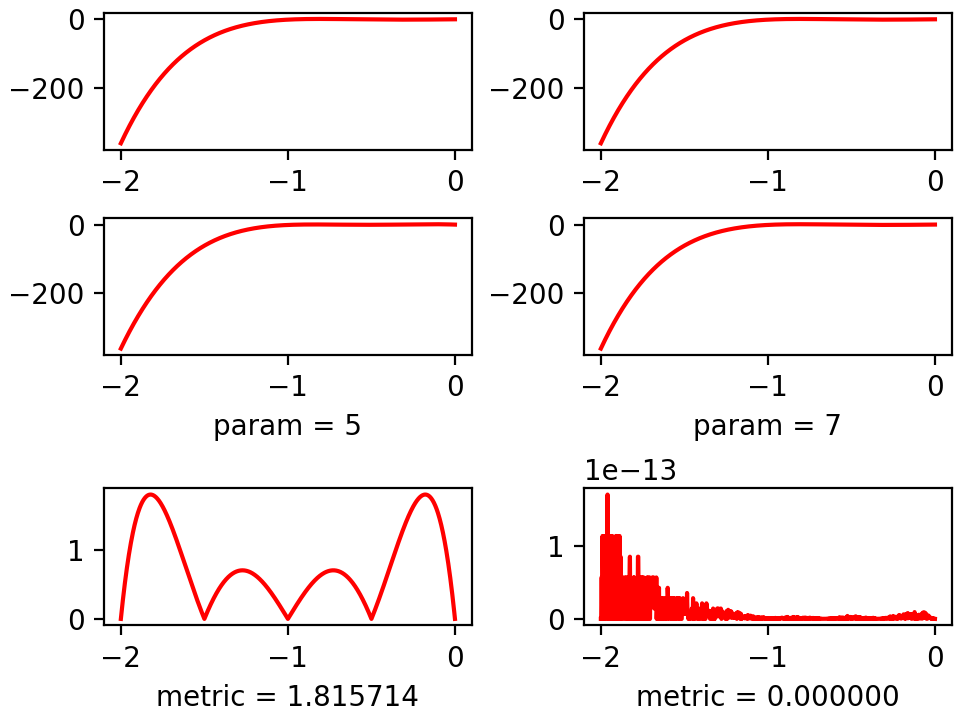
\includegraphics{F1_p5p7_Lagrange.png}
\captionsrussian[Рис. 1]{ Интерполяция функции (1)}
\hfill

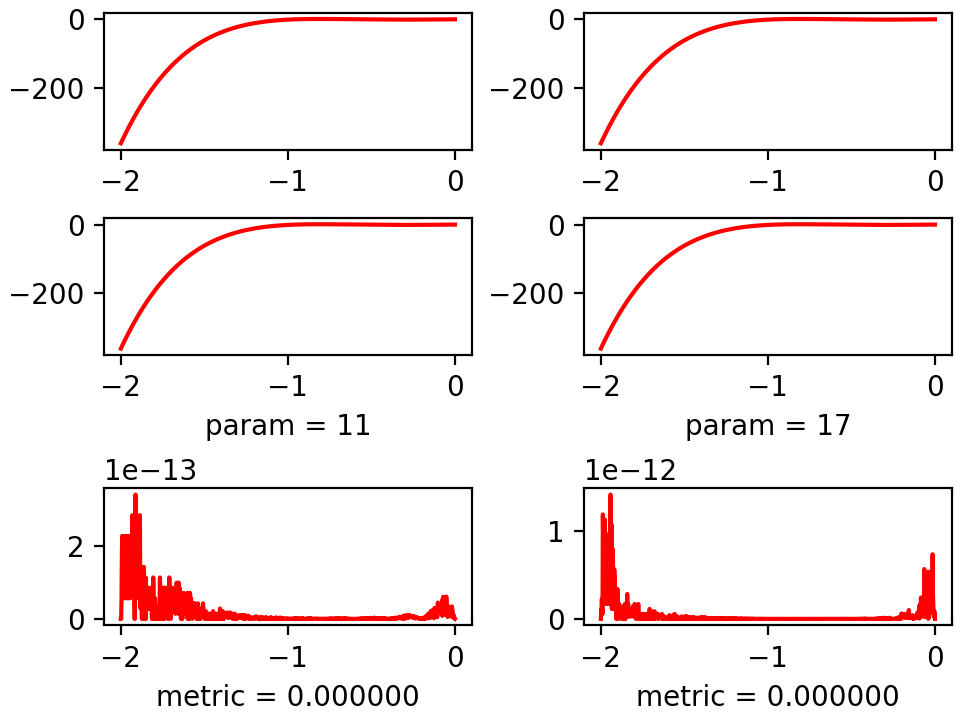
\includegraphics{F1_p11p17_Lagrange.png}
\captionsrussian[Рис. 2]{ Интерполяция функции (1)}
\hfill

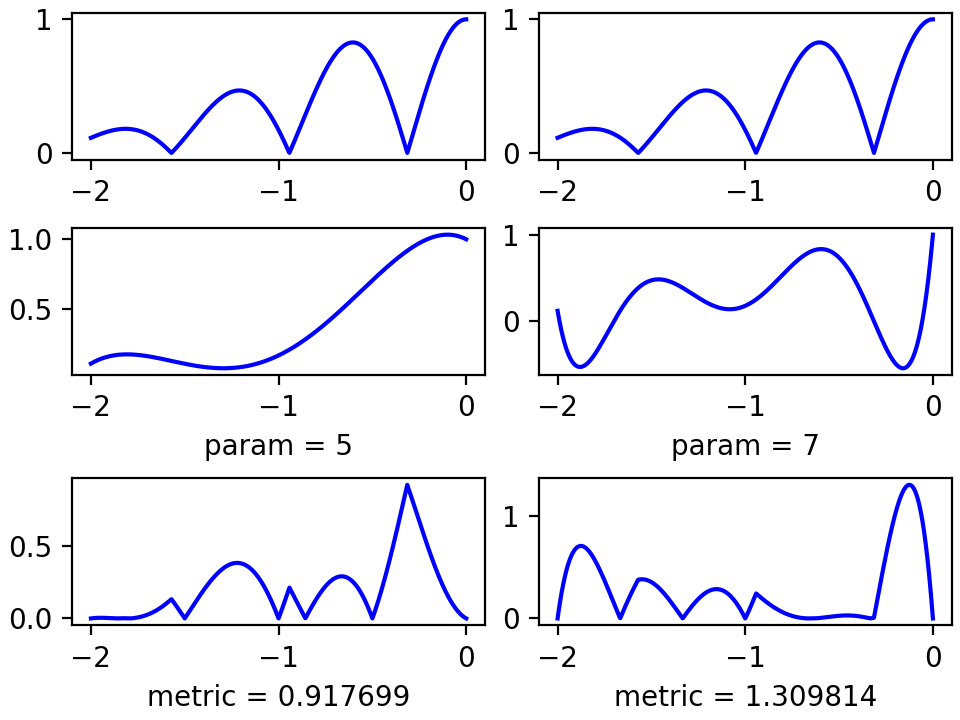
\includegraphics{F2_p5p7_Lagrange.png}
\captionsrussian[Рис. 3]{ Интерполяция функции (2)}

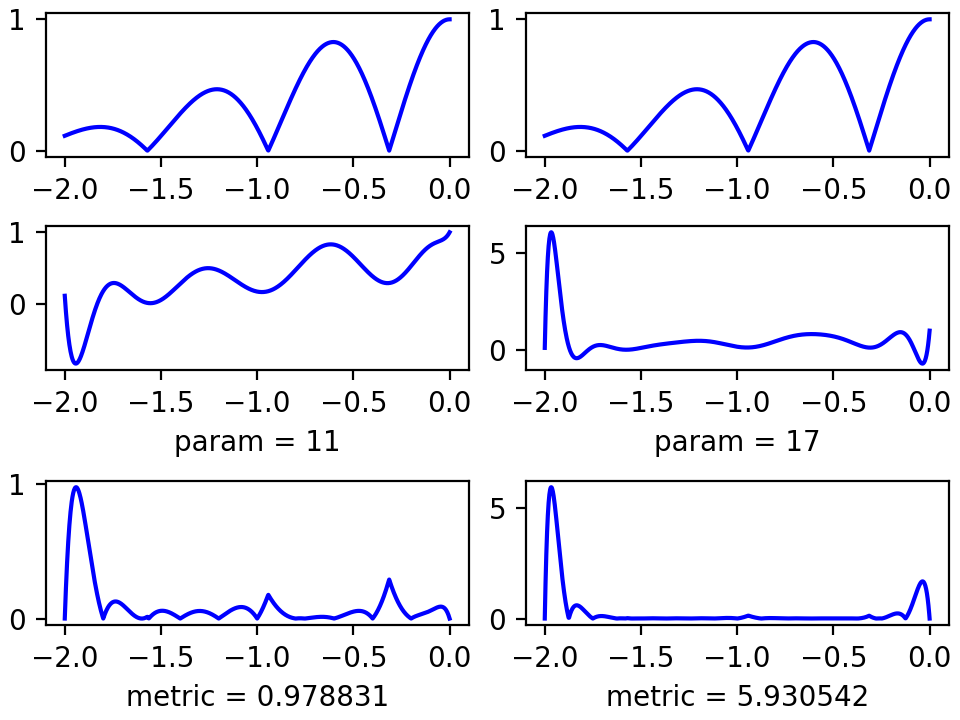
\includegraphics{F2_p11p17_Lagrange.png}
\captionsrussian[Рис. 4]{ Интерполяция функции (2)}

\begin{center}
	
	\begin{tabular}{ c   c   c}
		& \(f_1(x)\) & \(f_2(x)\) \\
		n=5 & 1.86 & 0.92 \\ 
		n=7 & 0.00 & 1.31 \\  
		n=11 & 0.00 & 0.98 \\
		n=17 &  0.00 & 5.93
	\end{tabular}
	
	\captionsrussian[Таблица 1.]{ Максимальные отклонения интерполянтов от функций.}
\end{center}
\end{Center}

\subsection{Приближение сплайнами}
\begin{Center}
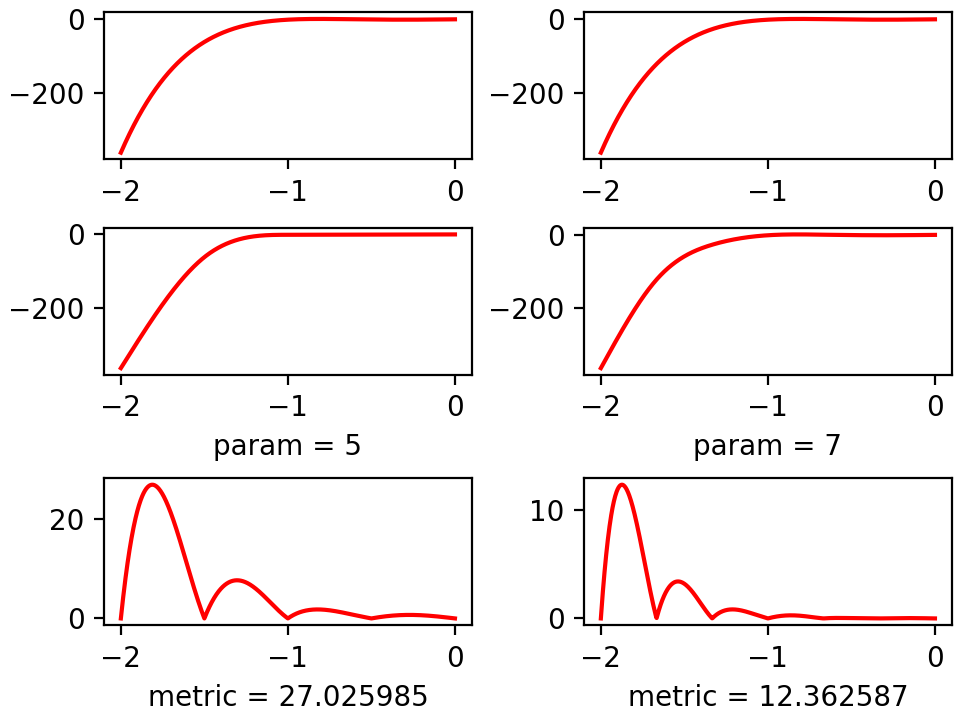
\includegraphics{F1_p5p7_Splain.png}
\captionsrussian[Рис. 5]{ Интерполяция функции (1)}

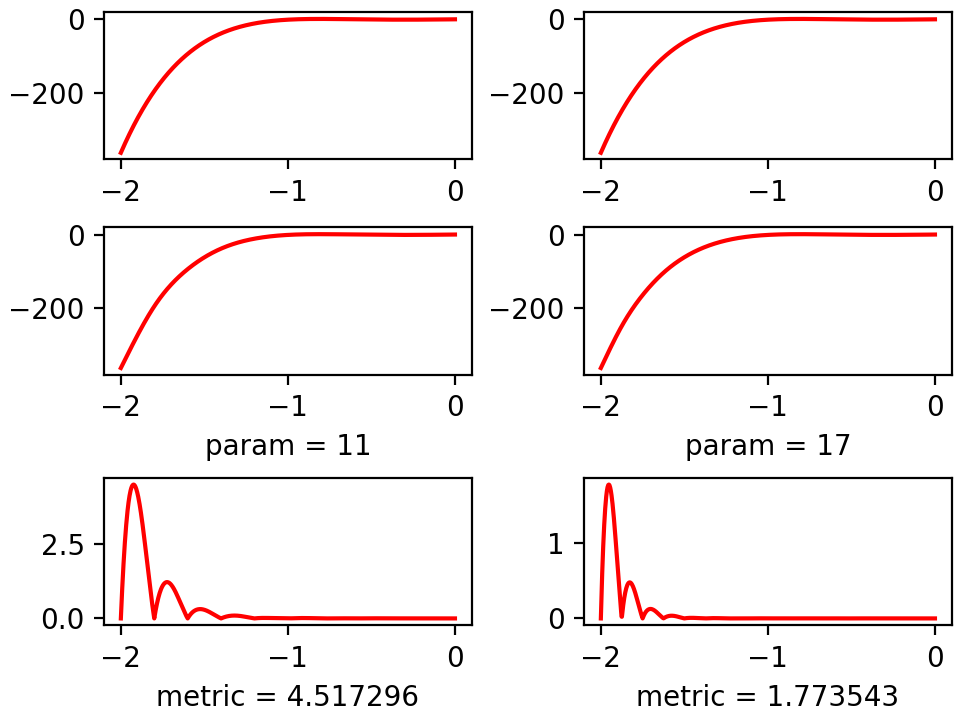
\includegraphics{F1_p11p17_Splain.png}
\captionsrussian[Рис. 6]{ Интерполяция функции (1)}

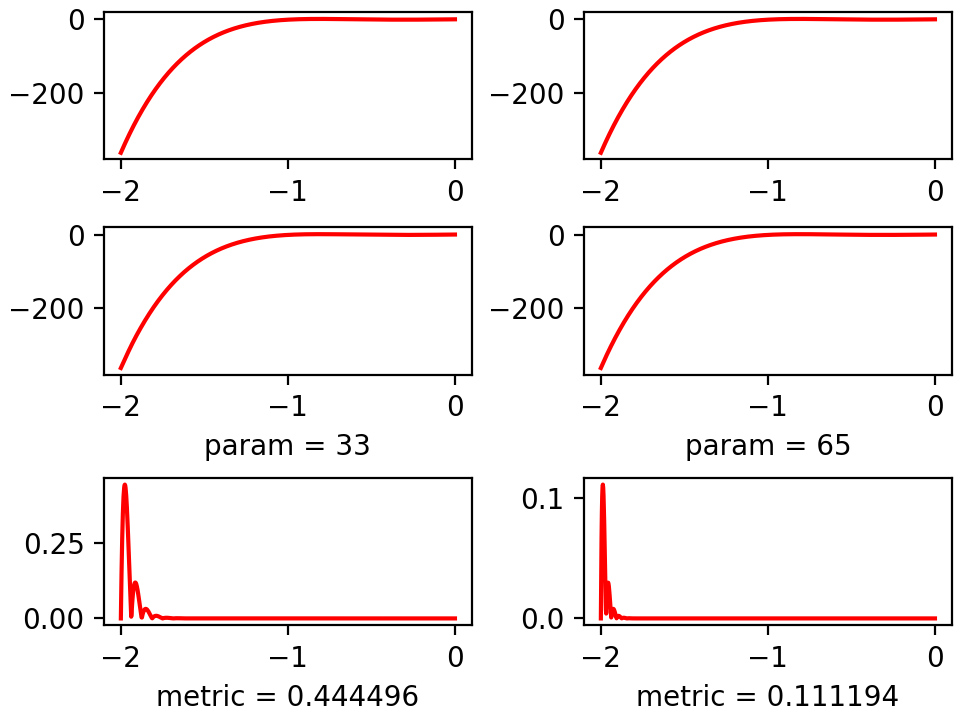
\includegraphics{F1_p33p65_Splain.png}
\captionsrussian[Рис. 7]{ Интерполяция функции (2)}

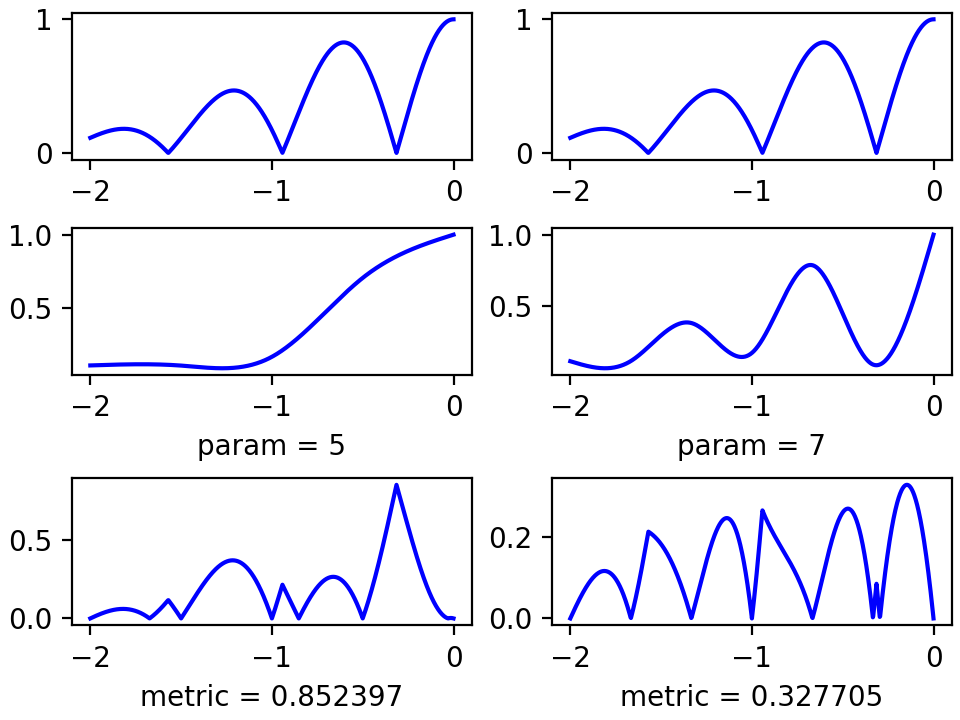
\includegraphics{F2_p5p7_Splain.png}
\captionsrussian[Рис. 8]{ Интерполяция функции (2)}

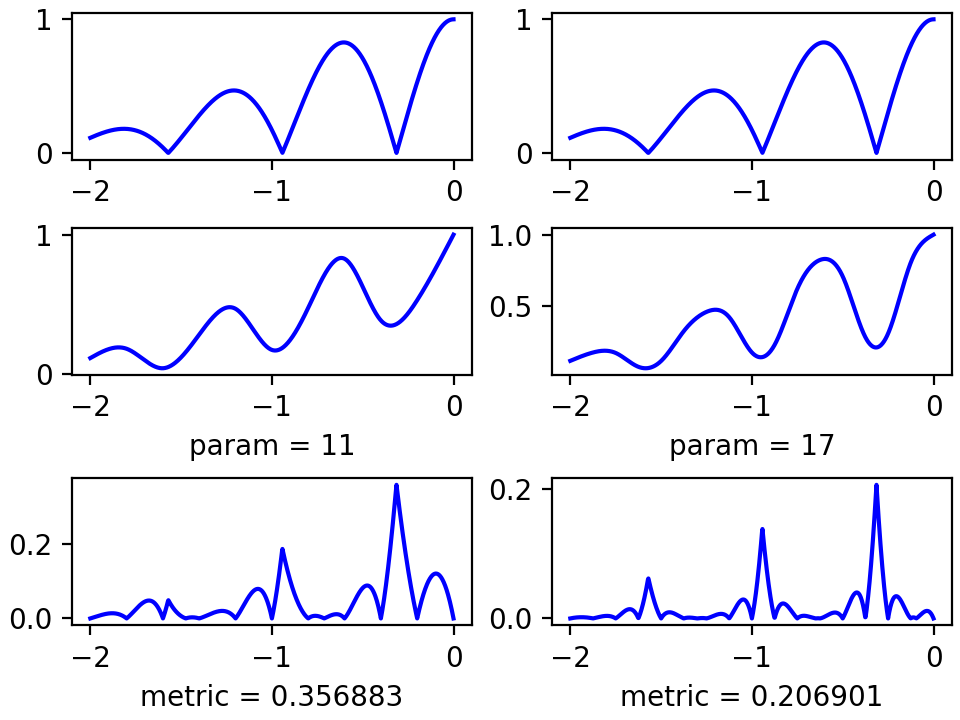
\includegraphics{F2_p11p17_Splain.png}
\captionsrussian[Рис. 9]{ Интерполяция функции (2)}

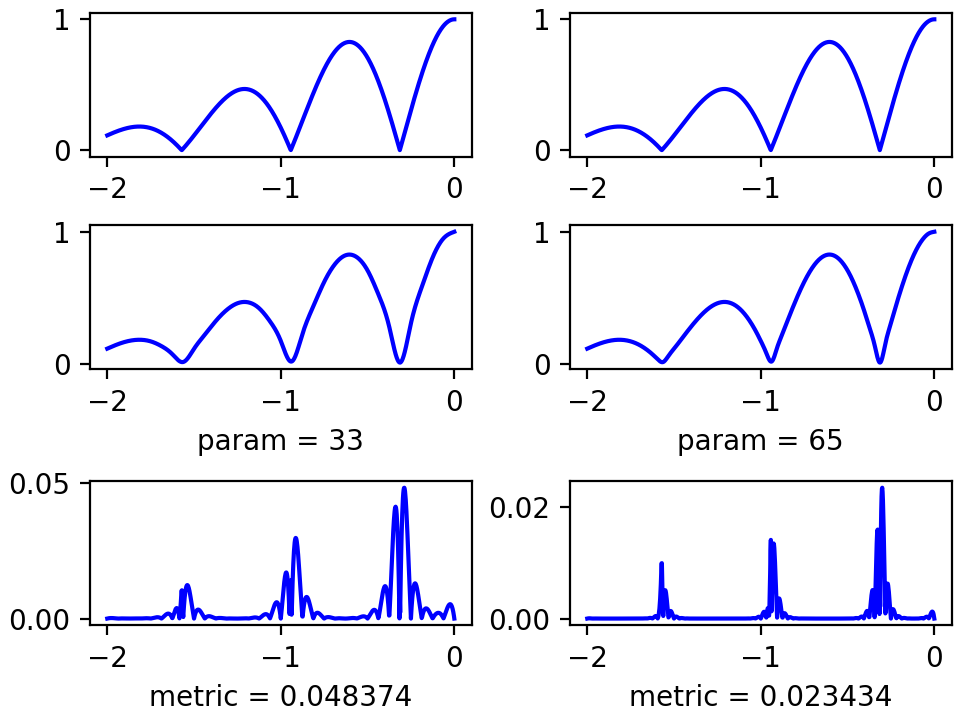
\includegraphics{F2_p33p65_Splain.png}
\captionsrussian[Рис. 10]{ Интерполяция функции (2)}
\end{Center}

\begin{center}
	
	
	\begin{tabular}{ c   c   c}
		 & \(f_1(x)\) & \(f_2(x)\) \\
		n=5 & 27.03 & 0.83 \\ 
		n=7 & 12.36 & 0.33 \\  
		n=11 & 4.52 & 0.36 \\
		n=17 &  1.77 & 0.21 \\
		n=33 & 0.44  & 0.05 \\
		n=65 & 0.11 & 0.02
	\end{tabular}
	
	\captionsrussian[Таблица 2.]{ Максимальные отклонения интерполянтов от функций.}
\end{center}


\subsection{Комментарии к графикам}
В 1 строке представлены изначальные функции \(f_i(x)\).
В 2 строке представлены их приближения \(F_i(x)\).
В 3 строке представлена функция \(g(x) = |f_i(x) - F_i(x)|\)

На графиках параметр {\large param} означает количество узлов в равномерной сетке, по которой проходила интерполяция. Значение {\large metric} показывает максимальное отклонение интерполянта от функции на равномерной сетке из 1000 узлов.

\subsection{Наблюдения}
Метод интерполяции многочленами Лагранжа позволяет хорошо приближать многочлены, как видим, уже на сетке из 7 узлов, мы полностью вычислили функцию (1). На рис. 1 видно, что максимальное отклонение на сетке из 5 узлов равно \(1.8147\), а на сетке из 7 узлов равно \(0.00\), на рис. 2 на сетках из 11 и 17 узлов максимальное отклонение равно \(0.00\) и \(0.00\), соответственно.
При этом мы совершенно не можем приблизить функцию (2).
Видно, что на рис. 3 на сетке из 5 узлов ошибка составляет \(0.9177\), а на сетке из 7 узлов уже \(1.3098\), на рис. 4 на сетке из 11 и 17 узлов \(0.9788\) и \(5.9305\), соответственно.

Метод интерполяции сплайнами показывает себя лучше в задаче интерполяции функции (2), чем метод (1), к примеру, на рис. 9 на сетке из 17 узлов ошибка доходит до \(0.2069\), что улучшает результат метода (1) почти в 25 раз, при этом метод (2) даёт худший результат при интерполяции функции (2), так на рис. 6 видно, что на сетке из 17 узлов ошибка достигает \(1.7735\).

\subsection{Программная реализация}
Данные численные методы реализованы на языке Python с использованием NumPy, matplotlib.

Код хранится в репозитории: 
https://github.com/GoodDay-lab/practicum-numerical-method

\section{Выводы}
Таким образом, в ходе выполнения задания был реализован метод приближения полиномами Лагранжа и кубическими сплайнами. Было отмечено и теоретически доказано, что полиномы Лагранжа могут эффективно приближать функции \(f \in C^n[a,b]\), давая достаточно хорошую оценку. При этом совершенно неопределенно поведение для негладких функций, и как мы видим, их они могут и вовсе не приближать. В таком случае можно использовать приближение сплайнами - кусочно-полиномиальными функциями. В этом случае оценка становится в разы лучше для негладких функций.


\section{Библиография}
\begin{enumerate}
    \item Хайкин С. "Нейронные сети. Полный курс", стр.82
    \item (url: https://education.yandex.ru/handbook/ml/article/mashinnoye-obucheniye)
    \item Тыртышников Е.Е. "Методы численного анализа", гл.12,13,14
    \item http://www.machinelearning.ru/wiki/
    \item А.А.Самарский, А.В.Гулин.  "Численные методы"
\end{enumerate}

\end{document}


